\documentclass[a4paper,12pt]{report}
% \usepackage{styles/fbe_tez}
\usepackage[utf8x]{inputenc}
\renewcommand{\labelenumi}{(\roman{enumi})}
\usepackage{amsmath, amsthm, amssymb}
\usepackage[bottom]{footmisc}
\usepackage{cite}
\usepackage{url}
\usepackage{graphicx}
\usepackage{longtable}
\usepackage{float}
\graphicspath{{figures/}}

\usepackage{multirow}
\usepackage{subfigure}
\usepackage{algorithm}
\usepackage{algorithmic}

\begin{document}

% Title Page
\title{CMPE 492 \\ Stablecoin Flow Analysis on Blockchains}
\author{
Celil \"{O}zkan \\
\\ \\
Advisor: \\
Prof. Can \"{O}zturan
}
\date{\today}
\maketitle{}
\pagenumbering{roman}
\tableofcontents

% ============================================================
\chapter{INTRODUCTION}
\pagenumbering{arabic}

\section{Broad Impact}

Stablecoins have become a critical infrastructure component in digital finance. They are widely
used for cross-border settlement, centralized exchange (CEX) operations, decentralized exchange
(DEX) liquidity provision, lending protocols, and cross-chain bridge transfers. As stablecoin
activity spans multiple blockchain networks, understanding how value flows and which entities act
as major hubs is important for both technical and economic analysis.

This project, named \textbf{ChainFlow}, builds a complete, end-to-end data pipeline and
interactive dashboard for analyzing stablecoin transfer flows across EVM-compatible blockchains.
Starting from raw on-chain event logs, the system collects transfer data, classifies addresses into
entity types, constructs directed weighted graphs, computes PageRank-based influence scores, and
exposes everything through an interactive web dashboard. A particular novelty is the inclusion of
\textit{x402 AI agent} classification -- tracking autonomous payment-capable agents defined
by the x402 protocol as a distinct entity class in the ecosystem.

Potential impact areas include:
\begin{itemize}
\item Measuring concentration of liquidity and systemic dependency on specific protocols.
\item Identifying major transfer corridors between users, exchanges, bridges, and protocol contracts.
\item Supporting transparent research on cross-network asset movement.
\item Tracking the emergence of autonomous AI agents making on-chain stablecoin payments.
\item Providing a practical and reproducible pipeline for blockchain data engineering and research.
\end{itemize}

Overall, ChainFlow contributes to improving the observability of decentralized financial systems,
which is increasingly important as these systems continue to grow in scale and influence.

\section{Ethical Considerations}

This project uses only publicly available on-chain data, including transaction logs and metadata.
No attempt is made to deanonymize blockchain addresses or associate them with real-world identities.
Address classification is limited to high-level categories such as exchanges (CEX), bridges, and
AI agents, without identifying individual persons.

Despite relying on public data, several ethical considerations arise:

\begin{itemize}
\item \textbf{Misclassification risk:} Address labels (e.g., CEX, Bridge) may be incomplete or
outdated, leading to incorrect interpretations.
\item \textbf{Attribution risk:} A single wallet address may represent multiple actors or automated
systems, so behavioral conclusions must remain probabilistic rather than definitive.
\item \textbf{Privacy considerations:} Although blockchain data is publicly accessible, large-scale
aggregation and analysis can reveal behavioral patterns. Care is taken to avoid conclusions that
could harm individuals or entities.
\item \textbf{No personal identification:} The system does not attempt to infer or expose real-world
identities behind addresses.
\item \textbf{Method transparency:} All assumptions, filtering decisions, and limitations are clearly
documented to ensure responsible interpretation of results.
\end{itemize}

To mitigate these risks, the project preserves exact chain and log identifiers, emphasizes
reproducibility, and keeps analysis at the network and protocol level rather than focusing on
individual actors.

% ============================================================
\chapter{PROJECT DEFINITION AND PLANNING}

\section{Project Definition}

The objective is to build a modular, end-to-end system that collects stablecoin transfer events
from multiple blockchains, classifies the participating addresses, constructs transaction flow
graphs, and provides interactive tools for exploration.

\textbf{Implemented scope:}
\begin{itemize}
\item \textbf{Networks:} Ethereum, Polygon, Arbitrum, Avalanche, Optimism.
\item \textbf{Tokens:} USDT, USDC, DAI (all networks), XAUT (Ethereum only).
\item \textbf{Data source:} Infura JSON-RPC (\texttt{eth\_getLogs}, \texttt{eth\_blockNumber}).
\item \textbf{Storage:} PostgreSQL 16 with partitioned \texttt{transfers} table, progress tracking,
PageRank score/edge tables, and materialized views for aggregation.
\item \textbf{Classification:} Four address classification categories applied to all stored
transfers: (i) \textit{CEX} -- known centralized exchange hot-wallet addresses retrieved via
per-network \textbf{Dune Analytics} queries (query IDs per chain); (ii) \textit{Bridge} --
bridge deposit and withdrawal contract addresses also retrieved from dedicated
\textbf{Dune Analytics} queries and cached in per-network YAML files; (iii) \textit{Mint/Burn}
-- detected directly from the transfer record when \texttt{from\_address} or \texttt{to\_address}
equals the EVM zero address, requiring no external lookup; (iv) \textit{x402 AI Agent} --
contract addresses registered as x402-enabled in the \textbf{8004scan.io} public agent
registry, fetched via its paginated REST API and cached in per-network YAML files.
\item \textbf{Graph analysis:} Directed weighted transfer graphs per network/token; PageRank
computed using NetworkX and persisted to the database.
\item \textbf{Dashboard:} FastAPI web application (ChainFlow) with three interactive tools:
PageRank Explorer, Flow Explorer, and Ecosystem Overview.
\end{itemize}

\section{Project Planning}

The implementation was organized in three phases:

\begin{enumerate}
\item \textbf{Fetch Phase (complete):} Build and validate robust event extraction and database
storage.
\item \textbf{Analysis Phase (complete):} Address classification (CEX, Bridge, Mint/Burn, x402
agents) and graph construction with PageRank.
\item \textbf{Reporting Phase (complete):} Interactive web dashboard, materialized views for
aggregated analytics, and final documentation.
\end{enumerate}

\subsection{Project Time and Resource Estimation}

Within the semester timeline, the main effort was distributed as follows:

\begin{itemize}
\item 20\%: Architecture decisions (schema design, network/token selection, data source selection).
\item 40\%: Core implementation (fetcher, classification, graph engine, CLI command flow).
\item 25\%: Web dashboard and materialized view design.
\item 15\%: Validation, debugging, and documentation.
\end{itemize}

Main resources:

\begin{itemize}
\item Python ecosystem: \texttt{requests}, \texttt{click}, \texttt{psycopg2}, \texttt{pyyaml},
\texttt{dotenv}, \texttt{networkx}, \texttt{fastapi}, \texttt{uvicorn}.
\item PostgreSQL 16 deployed via Docker.
\item Infura RPC endpoints for blockchain event retrieval.
\item Dune Analytics API for CEX address lists.
\item 8004scan.io API for x402 AI agent registry.
\end{itemize}

\subsection{Success Criteria}

The project defines the following success criteria:

\begin{itemize}
\item Correctly fetch and decode ERC-20 \texttt{Transfer} logs for selected tokens.
\item Support both automatic and manual block-range execution via CLI.
\item Store events in a relational schema with conflict-safe insertion.
\item Ensure resumability and traceability through chunk-level fetch progress records.
\item Classify addresses into CEX, Bridge, Mint/Burn, and x402 agent categories.
\item Compute and persist PageRank scores for each network and token combination.
\item Serve an interactive web dashboard exposing graph, wallet, and ecosystem views.
\end{itemize}

All criteria have been met. The system holds over 3.4 million transfer events across five networks.

\subsection{Risk Analysis}

Key technical and project risks include:

\begin{itemize}
\item \textbf{RPC result cap (10k logs):} Mitigated through adaptive chunk resizing when the
provider returns range overflow errors.
\item \textbf{Rate limits / provider dependency:} Reduced by migrating from explorer APIs to Infura
RPC and using controlled batch requests.
\item \textbf{Data duplication:} Prevented via unique constraint \texttt{(tx\_hash, log\_index,
network)} and \texttt{ON CONFLICT DO NOTHING}.
\item \textbf{Classification coverage:} Addressed by combining Dune Analytics queries (CEX and
Bridge), zero-address field inspection (Mint/Burn), and the 8004scan.io registry (x402 AI agents).
Coverage is incomplete by design and treated as probabilistic.
\item \textbf{Stale x402 address lists:} Mitigated by providing a CLI command to refresh the agent
file from the live registry at any time.
\item \textbf{Graph scale:} PageRank is pre-computed and stored in the database; only the top-10,000
scoring nodes are retained to keep query performance practical.
\end{itemize}

\subsection{Team Work (if applicable)}

The project is implemented by a single student developer. Progress was guided through regular
advisor meetings and iterative feedback, with development organized into three milestones.

% ============================================================
\chapter{RELATED WORK}

This project is implementation-oriented and grounded in publicly available blockchain tooling and
research. Four related areas are particularly relevant.

\textbf{(1) Blockchain data providers and explorers.}
Explorer APIs such as Etherscan, Arbiscan, Polygonscan, Snowtrace, and Optimistic Etherscan
\cite{etherscan_docs, arbiscan, polygonscan, snowtrace, optimistic_etherscan} provide convenient
access but become restrictive at high volume due to rate limits and endpoint constraints.
JSON-RPC endpoints (e.g., Infura) provide lower-level access better aligned with event-centric
pipelines. Practical RPC usage patterns are documented by Sharma \cite{sharma2020} and the
official Ethereum JSON-RPC specification \cite{ethereum_jsonrpc}.

\textbf{(2) ERC-20 event-based analysis.}
Many token analytics workflows reconstruct transfer networks by parsing \texttt{Transfer} events
rather than tracing full transaction internals. The ERC-20 standard is defined in the original
Ethereum Improvement Proposal by Vogelsteller and Buterin \cite{erc20}. Empirical research
demonstrates that ERC-20 transaction networks can be analyzed effectively with graph methods for
structural insights and prediction tasks \cite{somin2020}.

\textbf{(3) Graph centrality and PageRank.}
The PageRank algorithm, originally proposed by Page et al.~\cite{pagerank1999} for ranking web
pages by link importance, is directly applicable to blockchain address graphs where directed
transfer edges carry weight proportional to token flow. This project uses NetworkX's
weighted PageRank implementation with a damping factor of 0.85 to rank addresses by structural
influence in the transfer network.

\textbf{(4) x402 protocol for autonomous AI agent payments.}
The x402 protocol \cite{x402} defines a machine-readable HTTP-based standard for AI agents to
autonomously make stablecoin payments. Addresses associated with x402-enabled contracts are
discoverable through the 8004scan.io registry. This project identifies such agents as a distinct
entity class within the transfer ecosystem, enabling analysis of the emerging role of AI-driven
financial activity on public blockchains.

Compared to existing tools and approaches, ChainFlow focuses on building a transparent and
reproducible pipeline that integrates data collection, classification, graph analytics, and
interactive visualization in a single self-contained system.

% ============================================================
\chapter{METHODOLOGY}

The methodology is a four-phase data engineering and analysis pipeline designed for
reproducibility and extensibility.

\textbf{Step 1 -- Configuration-driven design.}
Network metadata, RPC endpoints, token contract addresses, and decimal precision are stored in
YAML configuration files (\texttt{networks.yaml} and \texttt{tokens.yaml}). CEX and bridge
address lists are maintained in per-network YAML files. This design separates configuration from
code and allows the pipeline to support additional networks or tokens with minimal code changes.

\textbf{Step 2 -- Command-line interface and modular pipeline.}
The pipeline exposes a CLI using \texttt{Click} with four implemented command groups:
\begin{itemize}
    \item \texttt{fetch} -- fetch transfer logs from the blockchain (automatic / manual modes)
    \item \texttt{classify\_addresses} -- label transfers by entity type (CEX, Bridge, Mint/Burn)
    \item \texttt{classify\_agents} -- identify x402 AI agent addresses and flag their transfers
    \item \texttt{graph} -- build the transfer graph and compute PageRank scores
\end{itemize}
The FastAPI web server is launched separately and reads pre-computed results from the database.

\textbf{Step 3 -- Fetch logs with adaptive chunking.}
The fetcher retrieves \texttt{Transfer} events via Infura JSON-RPC (\texttt{eth\_getLogs}).
Adaptive block chunking adjusts the request size based on network activity and provider limits
(maximum 10,000 logs per request). If a request exceeds the limit, the chunk size is halved and
retried automatically. Fetch progress is stored in the \texttt{fetch\_progress} table to support
resumable execution and auditing.

\textbf{Step 4 -- Log decoding and normalization.}
Raw logs are decoded into structured records including block/transaction identifiers, timestamps,
token metadata, sender and receiver addresses, and decimal-normalized transfer value.

\textbf{Step 5 -- Incremental persistence in PostgreSQL.}
Decoded records are written in batches to the \texttt{transfers} table using conflict-safe upsert
operations. The table is partitioned by \texttt{network} and indexed across block number, address,
and token fields for efficient temporal and entity-centric queries.

\textbf{Step 6 -- Address classification.}
Each network is processed by three classifiers:
\begin{itemize}
    \item \textit{Mint/Burn:} transfers where \texttt{from\_address} or \texttt{to\_address} is the
    EVM zero address (\texttt{0x000...0}) are labeled as minting or burning events.
    \item \textit{CEX:} known centralized exchange hot-wallet addresses (sourced from Dune Analytics)
    are matched against \texttt{from\_address}/\texttt{to\_address} and labeled with
    \texttt{entity\_class = 'CEX'}.
    \item \textit{Bridge:} gateway and router contract addresses for cross-chain bridges (maintained
    in YAML config) are matched and labeled \texttt{entity\_class = 'BRIDGE'}.
\end{itemize}
Labels are stored as \texttt{TEXT[]} arrays on each transfer row, allowing multi-label assignment
where applicable.

\textbf{Step 7 -- x402 AI agent identification.}
Contract addresses registered as x402-enabled in the 8004scan.io registry are fetched via its
public API. The agent address list is cached to a YAML file and then used to flag transfers
originating from x402 agents (\texttt{is\_from\_x402 = true}). This boolean flag enables
independent segmentation from the CEX/Bridge entity classes.

\textbf{Step 8 -- Transfer graph construction and PageRank.}
For each network (optionally filtered by token), aggregated transfer pairs are loaded from the
database as a directed weighted edge list. A directed graph $G = (V, E)$ is built using
NetworkX, where each edge $(u, v, w)$ represents the aggregate stablecoin flow from address
$u$ to address $v$:
\[
E = \{(u, v, w) \mid u = \text{from\_address},\; v = \text{to\_address},\; w = \sum \text{value} \}
\]
Weighted PageRank is computed with damping factor $\alpha = 0.85$:
\[
\text{PR}(v) = \frac{1 - \alpha}{|V|} + \alpha \sum_{u \in \text{in}(v)} \frac{\text{PR}(u) \cdot w(u,v)}{\sum_{k} w(u,k)}
\]
The top 10,000 scored nodes and their connecting edges are persisted to the
\texttt{pagerank\_scores} and \texttt{pagerank\_edges} tables.

\textbf{Step 9 -- Materialized views for aggregation.}
Four PostgreSQL materialized views pre-aggregate classification and x402 data for dashboard
queries: (i) segment-level volume and transaction counts, (ii) x402 token breakdown,
(iii) monthly x402 activity timeline, and (iv) top x402 agent leaderboard.

\textbf{Step 10 -- Interactive web dashboard.}
The ChainFlow dashboard is a FastAPI application serving three analysis tools:
\begin{itemize}
    \item \textit{PageRank Explorer:} a D3.js force-directed graph rendering the top-$N$ addresses
    colored by entity class, with interactive zoom, node inspection, and network/token filters.
    \item \textit{Flow Explorer:} a per-wallet view showing full inflow/outflow history, net balance,
    top counterparties by volume, and entity classification across networks and tokens.
    \item \textit{Ecosystem Overview:} a network-level breakdown of stablecoin volume and transaction
    share by segment (CEX, Bridge, x402 Agent, Regular Wallet), with the x402 monthly activity
    timeline and top agent leaderboard.
\end{itemize}

% ============================================================
\chapter{REQUIREMENTS SPECIFICATION}

The system requirements are divided into functional and non-functional parts. Use case and
activity diagrams are provided to visualize system interactions and the processing pipeline.

\section*{Functional Requirements}
\begin{enumerate}
    \item The system shall fetch ERC-20 \texttt{Transfer} logs for configured token contracts.
    \item The system shall support multiple EVM-compatible networks through a unified interface.
    \item The system shall provide both manual (user-defined block ranges) and automatic
    (resume from last processed block) fetching modes.
    \item The system shall decode and store transfer fields in a normalized PostgreSQL schema.
    \item The system shall prevent duplicate inserts using deterministic uniqueness constraints
    (\texttt{tx\_hash}, \texttt{log\_index}, \texttt{network}).
    \item The system shall store fetch-progress checkpoints for each processed block chunk to
    support resumable runs.
    \item The system shall classify transfer addresses into CEX, Bridge, and Mint/Burn categories.
    \item The system shall identify x402 AI agent addresses and flag associated transfers.
    \item The system shall construct a directed weighted transfer graph per network/token and
    compute PageRank influence scores.
    \item The system shall serve an interactive web dashboard for graph exploration, wallet
    flow analysis, and ecosystem overview.
\end{enumerate}

\section*{Non-Functional Requirements}
\begin{enumerate}
    \item \textbf{Reliability:} Interrupted or failed runs should be recoverable using stored
    progress checkpoints.
    \item \textbf{Scalability:} Database schema and indexes should support growth across multiple
    chains and high-volume token events.
    \item \textbf{Maintainability:} Configuration files should allow easy addition or removal of
    chains, tokens, and address lists without modifying core code.
    \item \textbf{Traceability:} Each stored event should preserve source identifiers
    (\texttt{tx\_hash}, \texttt{log\_index}, \texttt{block\_number}, \texttt{network}).
    \item \textbf{Usability:} Command-line interface and web dashboard should be simple to operate.
    \item \textbf{Performance:} PageRank and ecosystem queries should be served from
    pre-computed database results to ensure sub-second dashboard response times.
\end{enumerate}

\section*{Primary Use Cases}

\begin{figure}[H]
    \centering
    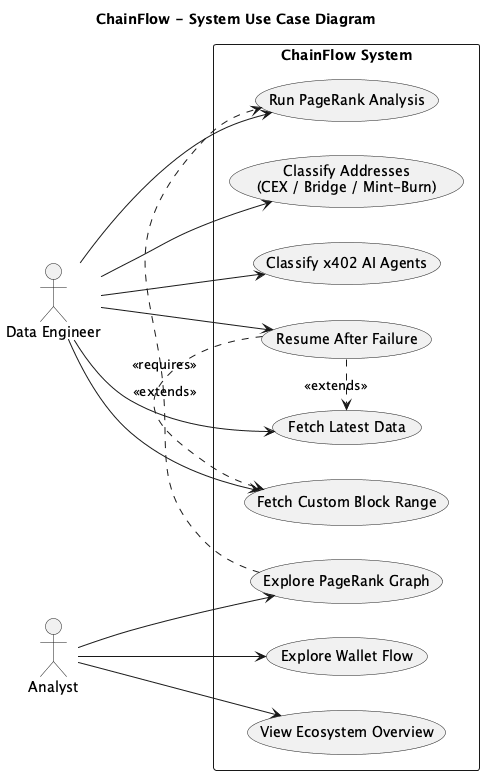
\includegraphics[width=0.75\textwidth,height=0.55\textheight,keepaspectratio]{figures/use_case_fetch.png}
    \caption{Use Case Diagram: ChainFlow System}
    \label{fig:uc}
\end{figure}

\begin{itemize}
    \item \textbf{UC-1 Fetch Latest Data:} Data engineer starts automatic mode; the system
    fetches from the last processed block to the latest chain block.
    \item \textbf{UC-2 Fetch Custom Block Range:} Data engineer provides start/end block; the system
    fetches the specified range.
    \item \textbf{UC-3 Resume After Failure:} Data engineer re-runs fetch; the system avoids duplicates
    and continues from remaining chunks.
    \item \textbf{UC-4 Classify Addresses:} Data engineer triggers address classification; the
    system applies CEX, Bridge, and Mint/Burn labels to all stored transfers.
    \item \textbf{UC-5 Classify x402 Agents:} Data engineer fetches the x402 agent registry and
    flags matching transfers in the database.
    \item \textbf{UC-6 Run PageRank Analysis:} Data engineer runs the graph command; the system
    builds the transfer graph and saves scored nodes and edges to the database.
    \item \textbf{UC-7--9 Dashboard tools:} Analyst accesses PageRank Explorer, Flow Explorer,
    or Ecosystem Overview via the web browser.
\end{itemize}

% ============================================================
\chapter{DESIGN}

\section{Information Structure}

The database schema consists of four main tables and four materialized views.

\textbf{(1) transfers} (partitioned by \texttt{network})
\begin{itemize}
    \item \textbf{Keys and provenance:} \texttt{tx\_hash}, \texttt{log\_index}, \texttt{block\_number},
    \texttt{block\_hash}, \texttt{block\_timestamp}.
    \item \textbf{Flow fields:} \texttt{from\_address}, \texttt{to\_address}, \texttt{value},
    \texttt{raw\_value}.
    \item \textbf{Asset context:} \texttt{token\_symbol}, \texttt{token\_address}, \texttt{network}.
    \item \textbf{Classification fields:} \texttt{from\_entity\_class TEXT[]},
    \texttt{to\_entity\_class TEXT[]}, \texttt{is\_from\_x402 BOOL}, \texttt{is\_to\_x402 BOOL},
    \texttt{event\_class VARCHAR(32)}.
    \item \textbf{Integrity:} unique constraint on \texttt{(tx\_hash, log\_index, network)}.
\end{itemize}

\textbf{(2) fetch\_progress}
\begin{itemize}
    \item Stores processed chunk ranges and log counts per network.
    \item Unique on \texttt{(network, chunk\_start, chunk\_end)}.
\end{itemize}

\textbf{(3) pagerank\_scores}
\begin{itemize}
    \item Stores pre-computed PageRank scores per \texttt{(network, token\_symbol, address)}.
    \item Indexed on \texttt{(network, token\_symbol, score DESC)} for fast top-$N$ queries.
\end{itemize}

\textbf{(4) pagerank\_edges}
\begin{itemize}
    \item Stores directed edges between the top-ranked nodes for graph visualization.
    \item Unique on \texttt{(network, token\_symbol, from\_address, to\_address)}.
\end{itemize}

\textbf{Materialized Views:} \texttt{mv\_ecosystem\_segments} (volume/count by entity segment),
\texttt{mv\_ecosystem\_x402\_tokens} (x402 token breakdown), \texttt{mv\_ecosystem\_x402\_timeline}
(monthly x402 activity), and \texttt{mv\_ecosystem\_x402\_agents} (agent leaderboard) are
pre-aggregated at pipeline run time to support sub-second dashboard queries.

\begin{figure}[H]
    \centering
    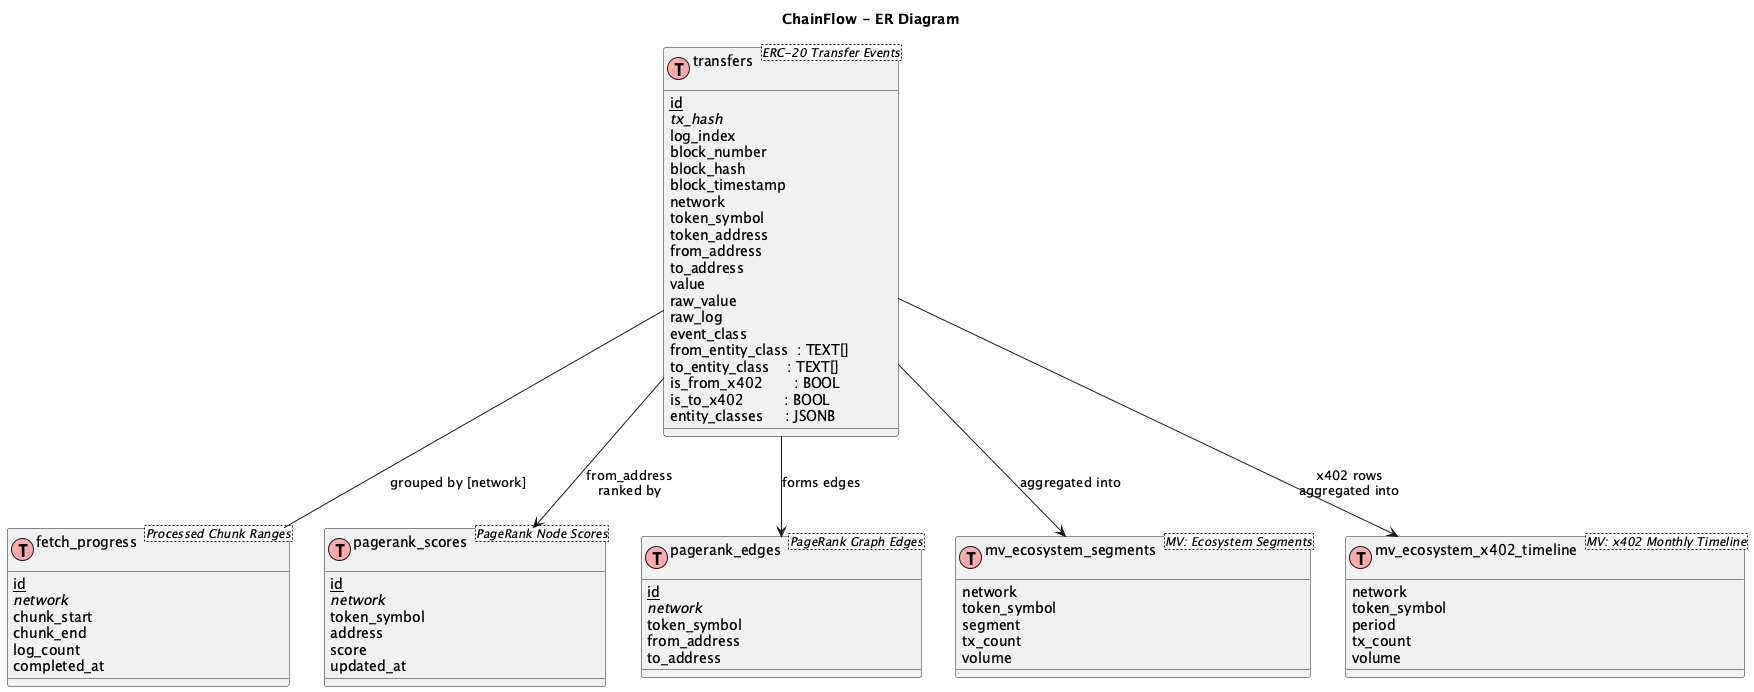
\includegraphics[width=0.95\textwidth]{figures/er_diagram.png}
    \caption{ER Diagram: ChainFlow Database Schema}
    \label{fig:er}
\end{figure}

\section{Information Flow}

The full data flow proceeds through four sequential phases, as illustrated in the activity diagram:

\begin{enumerate}
    \item \textbf{Fetch:} CLI requests \texttt{eth\_getLogs} for configured token addresses,
    decodes the results, and persists them incrementally to PostgreSQL.
    \item \textbf{Classify:} CLI runs address matching against CEX/Bridge/x402 label sources and
    updates entity class columns in the \texttt{transfers} table.
    \item \textbf{Graph:} CLI loads aggregated edges from the database, builds a directed weighted
    graph, computes weighted PageRank, and saves scores and edges back to the database.
    \item \textbf{Dashboard:} FastAPI reads pre-computed data from the database and serves
    interactive visualization pages to the browser.
\end{enumerate}

\subsection*{Activity Diagram}
\begin{figure}[H]
    \centering
    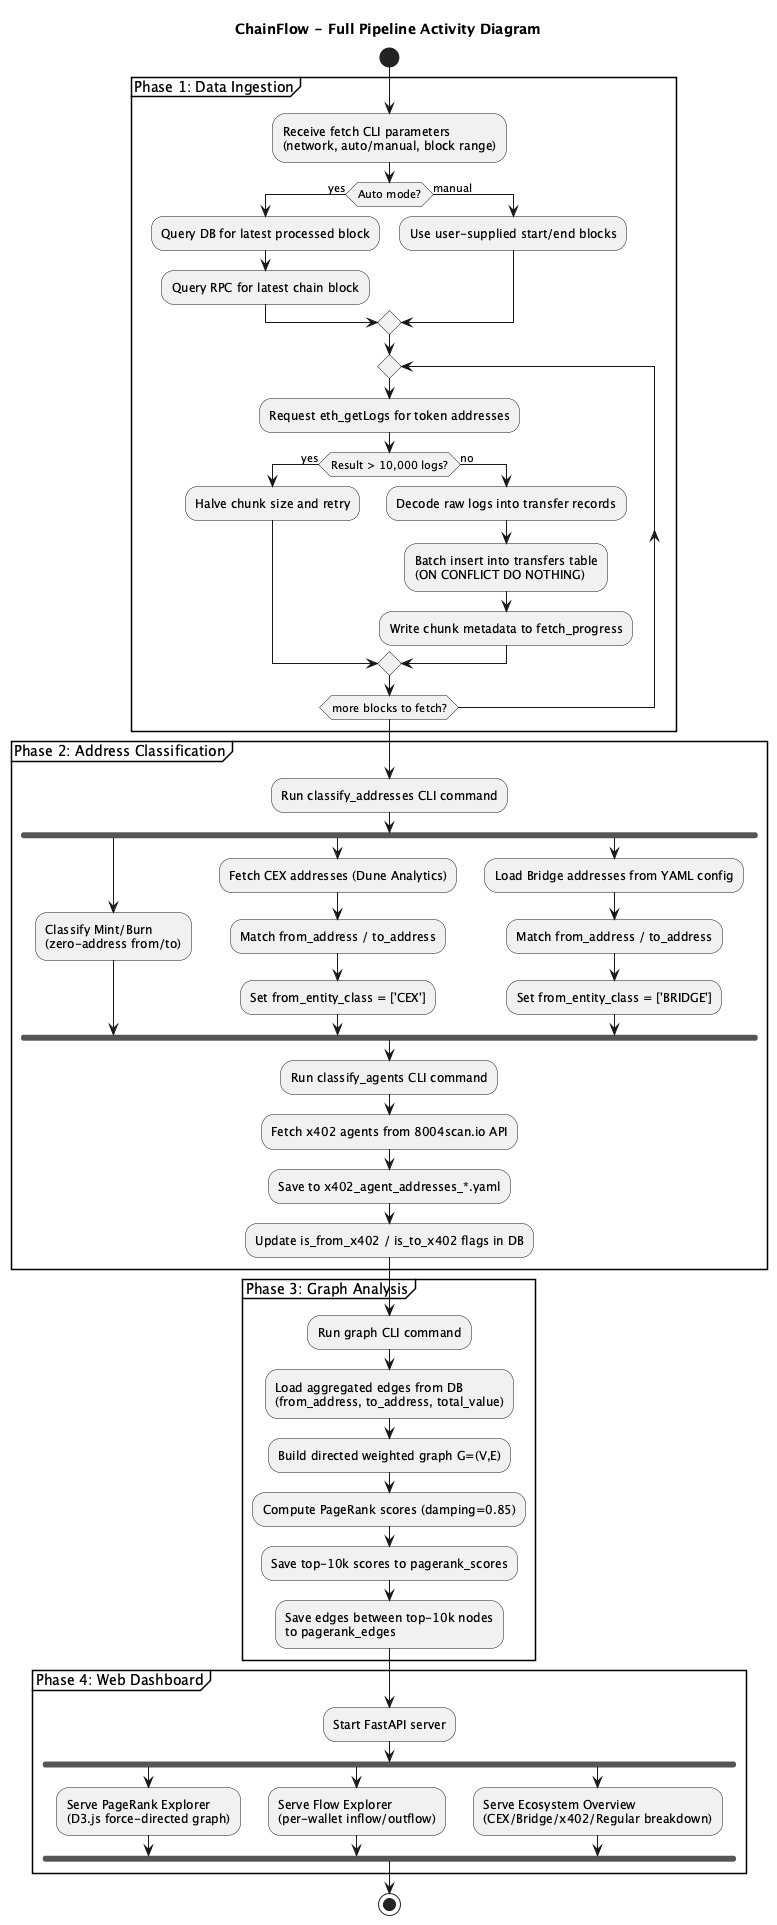
\includegraphics[width=0.95\textwidth,height=0.70\textheight,keepaspectratio]{figures/activity_diagram.png}
    \caption{Activity Diagram: Full ChainFlow Pipeline}
    \label{fig:activity}
\end{figure}

\subsection*{Sequence Diagram}
\begin{figure}[H]
    \centering
    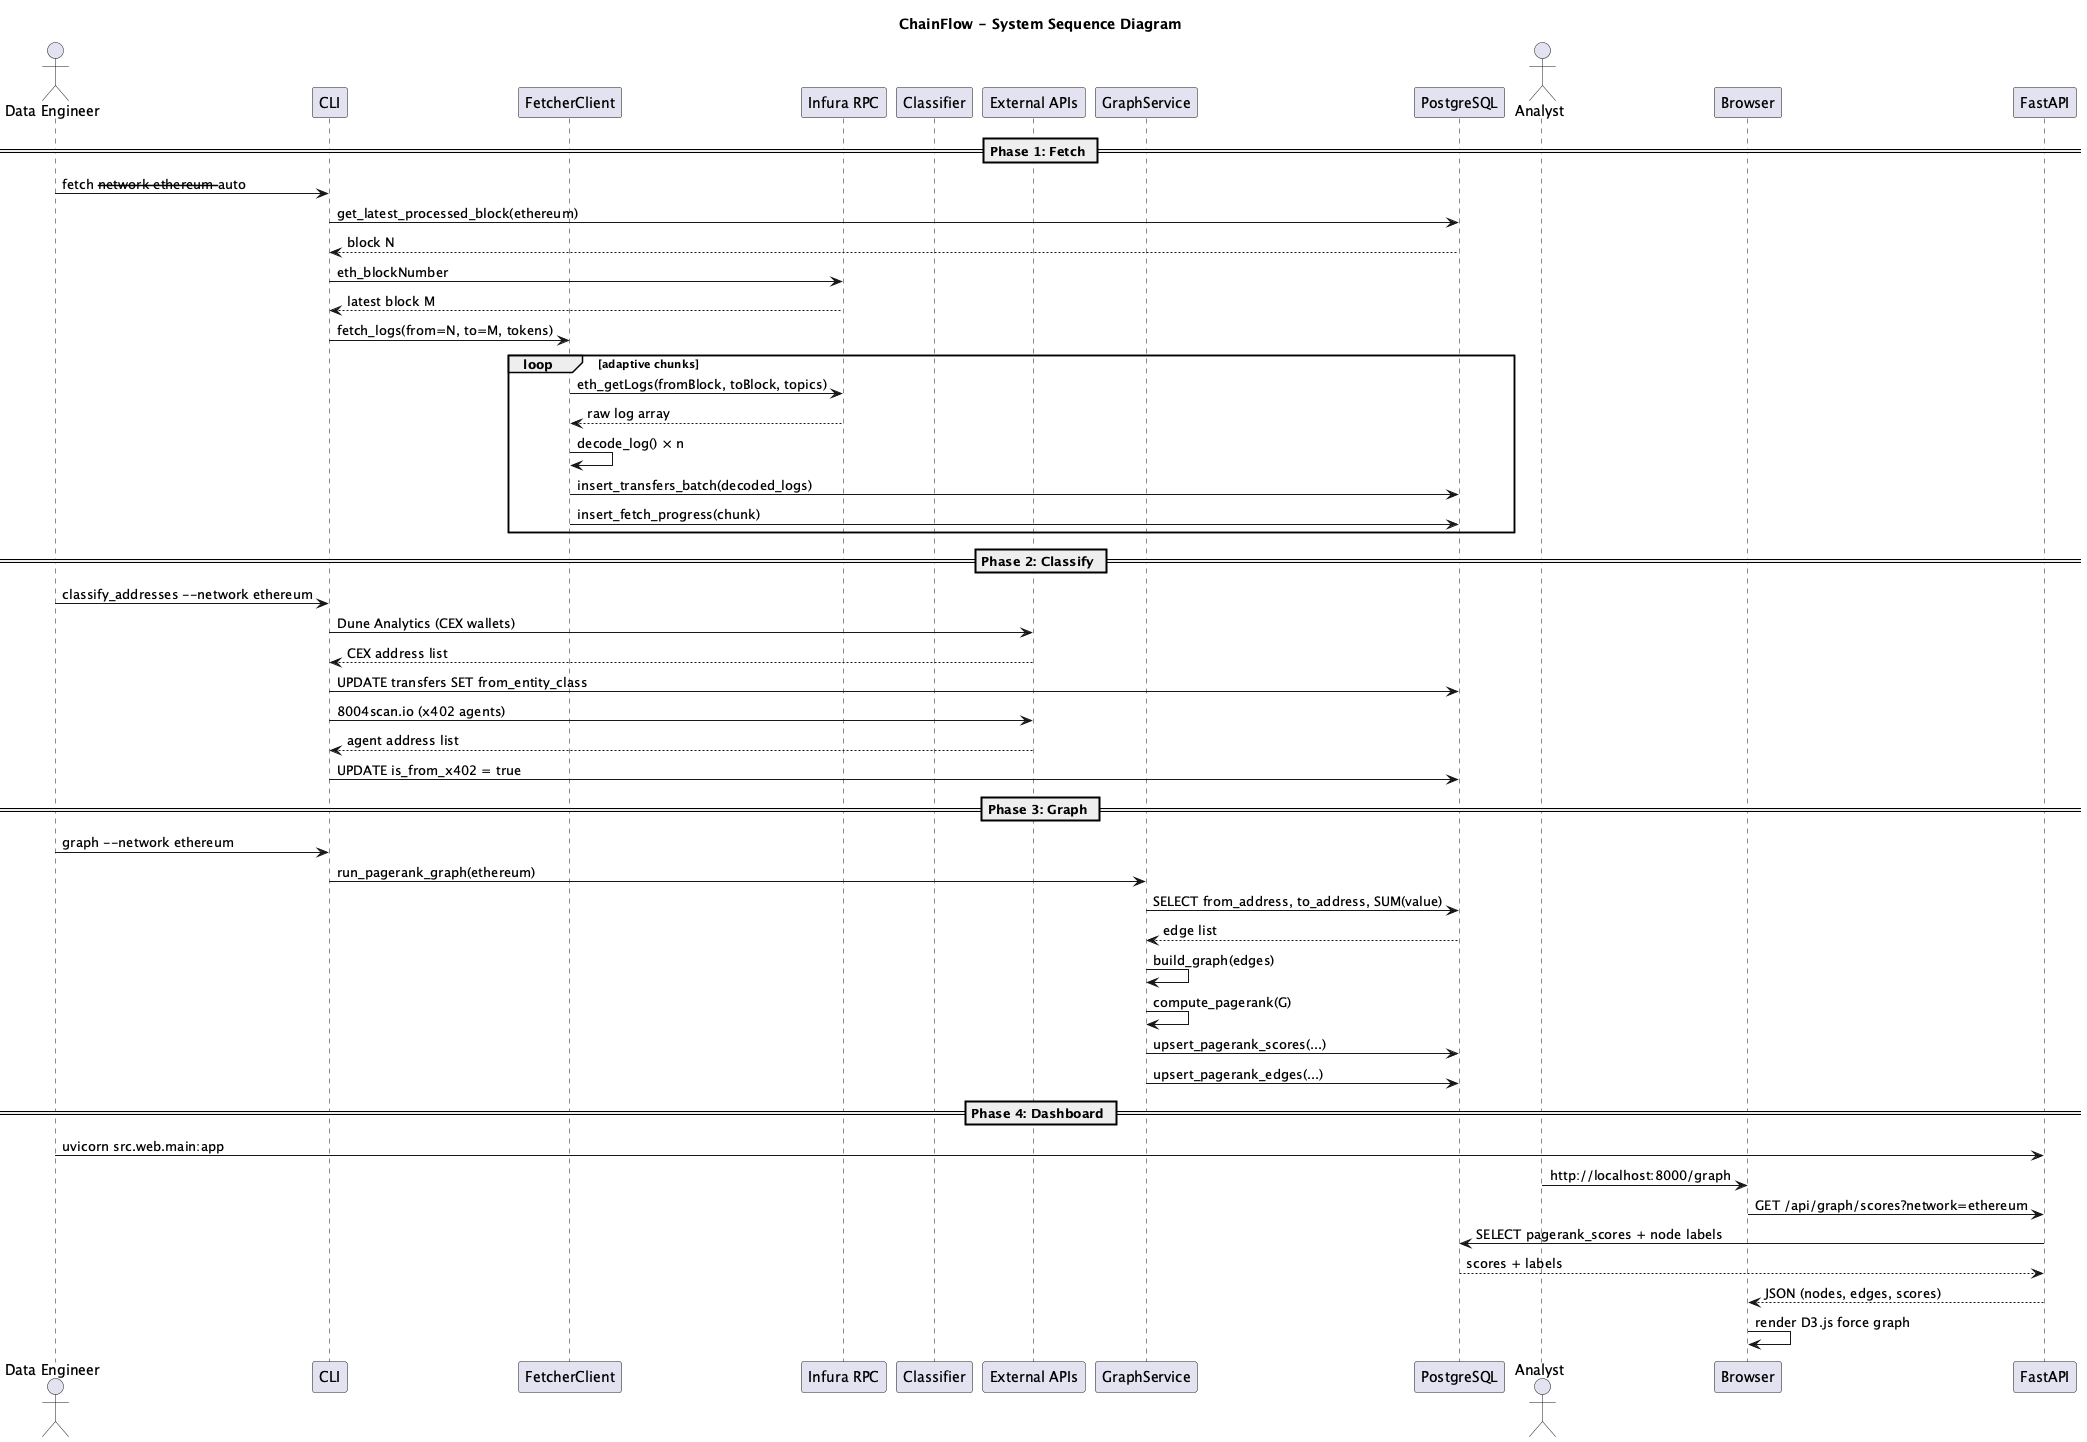
\includegraphics[width=0.95\textwidth]{figures/sequence_diagram.png}
    \caption{Sequence Diagram: End-to-End Data Flow from Fetch to Dashboard}
    \label{fig:sequence}
\end{figure}

\section{System Design Diagrams}

\begin{figure}[H]
    \centering
    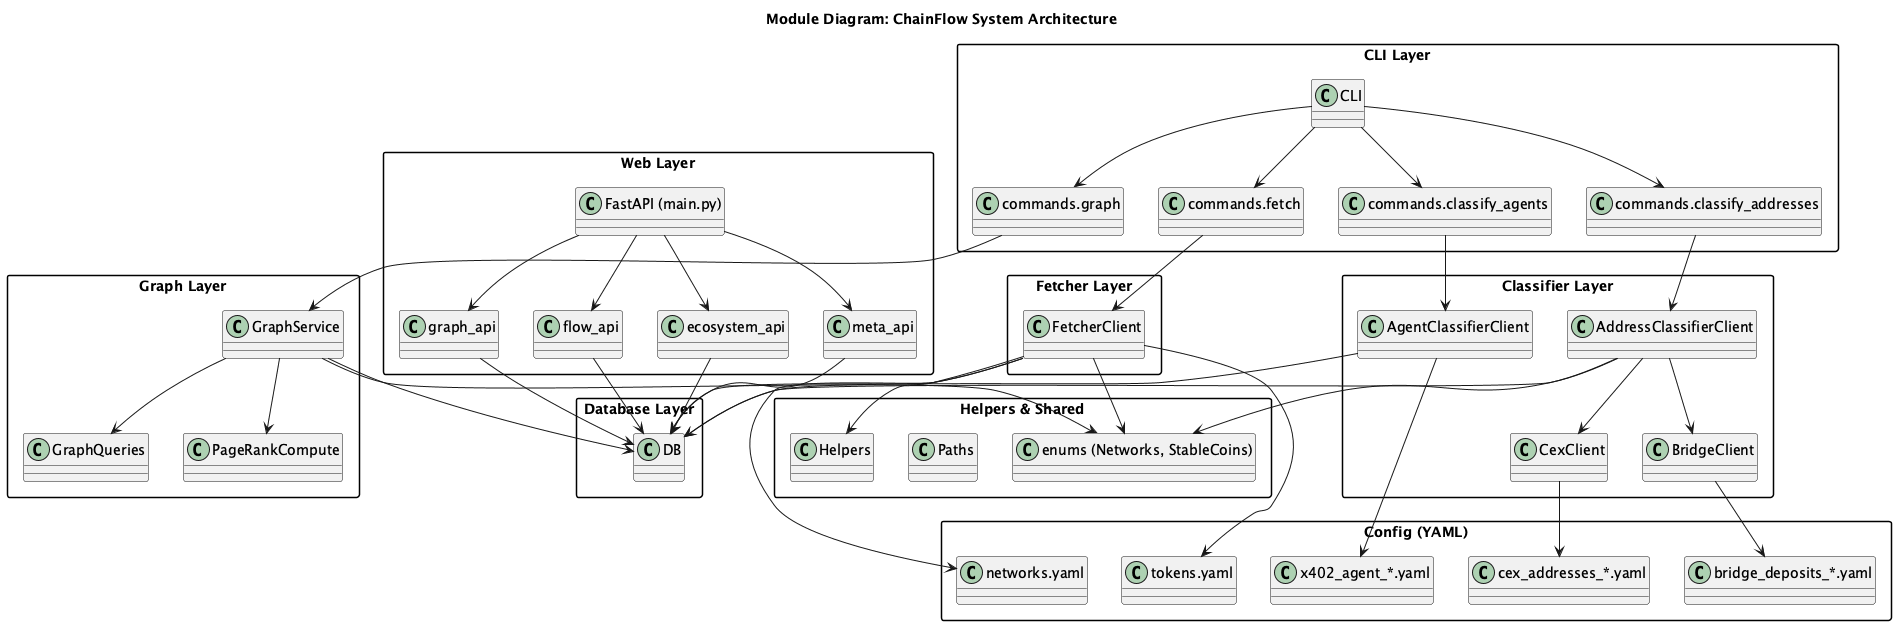
\includegraphics[width=0.95\textwidth]{figures/module_diagram.png}
    \caption{Module Diagram: ChainFlow Project Structure and Dependencies}
    \label{fig:module}
\end{figure}

\begin{figure}[H]
    \centering
    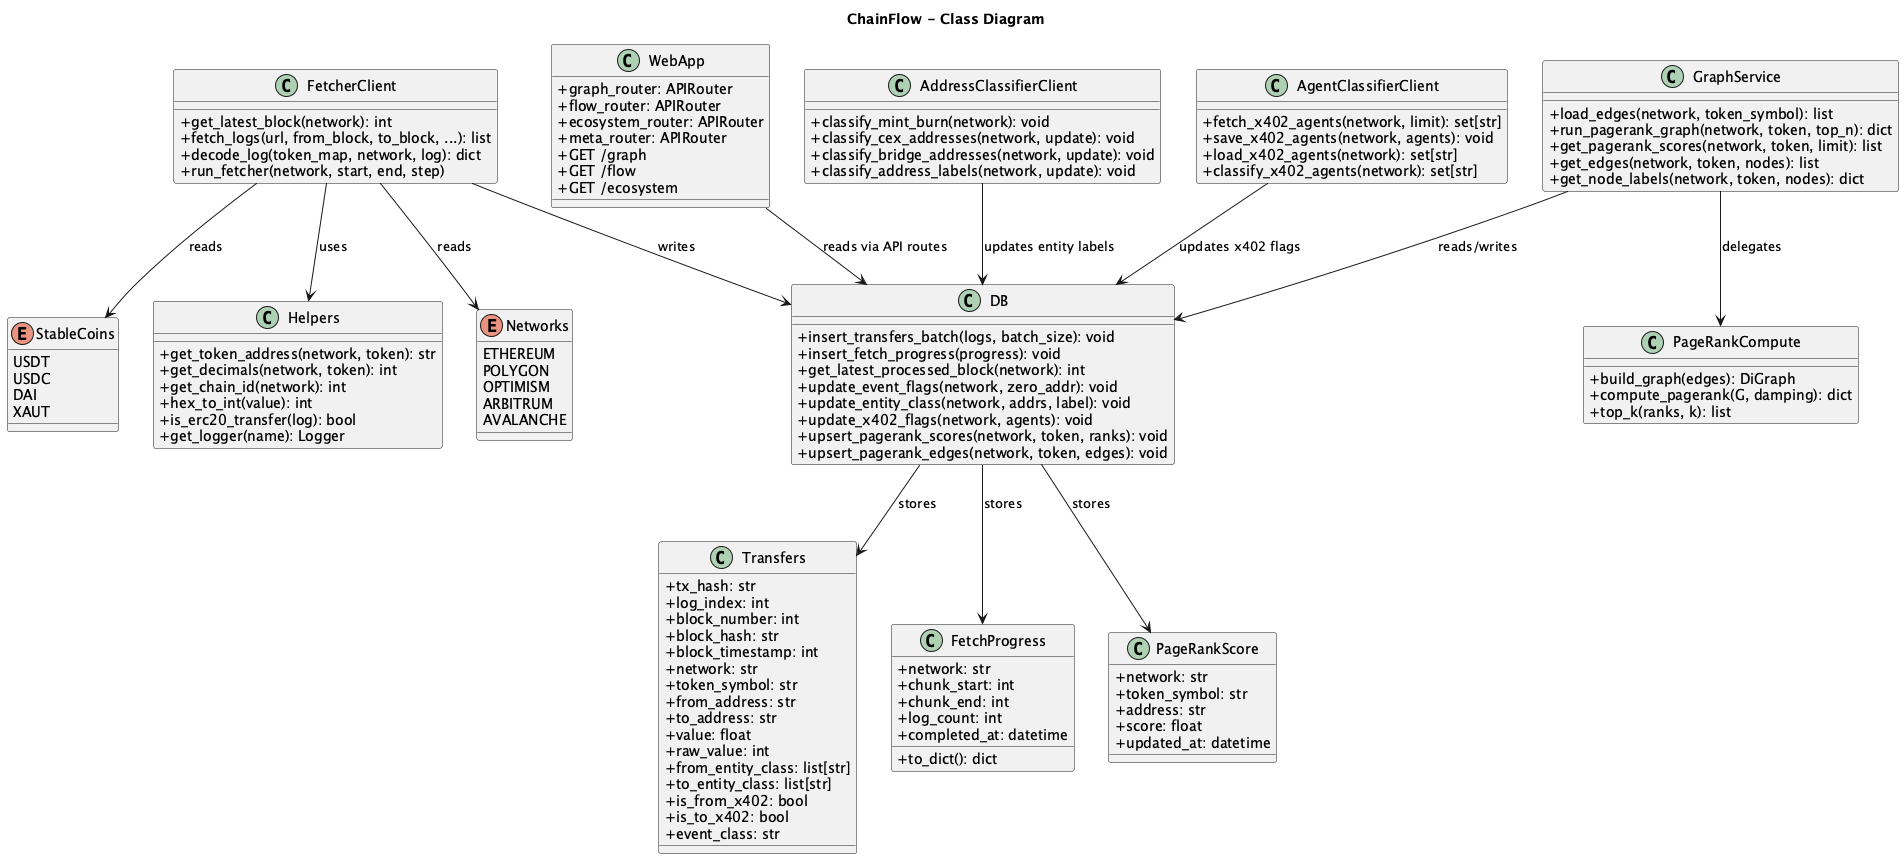
\includegraphics[width=0.95\textwidth]{figures/class_diagram.png}
    \caption{Class Diagram: Main Classes and Data Structures}
    \label{fig:class}
\end{figure}

\noindent
\textbf{Key design notes:}
\begin{itemize}
    \item \texttt{FetcherClient} handles RPC requests, log decoding, and adaptive chunking; it
    writes only to the database and has no dependency on any classifier or graph module.
    \item \texttt{AddressClassifierClient} is an orchestrator that delegates to \texttt{CexClient}
    and \texttt{BridgeClient}; it only issues \texttt{UPDATE} statements, never inserting rows.
    \item \texttt{AgentClassifierClient} handles the x402 classification path independently,
    including API pagination and YAML caching.
    \item \texttt{GraphService} reads edges from PostgreSQL, delegates computation to
    \texttt{PageRankCompute} (NetworkX), and writes results back to the database.
    \item The FastAPI web layer reads exclusively from pre-computed tables and materialized views,
    keeping read latency low and decoupled from pipeline execution.
\end{itemize}

\section{User Interface Design}

The current user interface has two components: a command-line interface for pipeline execution
and a web dashboard for interactive analysis.

\textbf{CLI:} The \texttt{Click}-based CLI exposes four commands:
\texttt{fetch}, \texttt{classify\_addresses}, \texttt{classify\_agents}, and \texttt{graph}.
Each command accepts a \texttt{--network} parameter and additional flags appropriate to its
function. The CLI is suitable for scheduling (cron, cloud VM, CI jobs) and integrates cleanly
with shell scripting.

\textbf{ChainFlow Web Dashboard:} The FastAPI application serves three views accessible from
the browser:
\begin{itemize}
    \item \textit{PageRank Explorer (\texttt{/graph}):} A D3.js force-directed graph showing the
    top-$N$ addresses. Node size encodes PageRank score; color encodes entity type (CEX, Bridge,
    x402 Agent, or Regular Wallet). Users can filter by network and token, zoom/pan the graph,
    and click nodes to inspect address details.
    \item \textit{Flow Explorer (\texttt{/flow}):} A wallet-centric view. Users enter any address
    to see its complete transfer history, aggregate inflow and outflow per token, top counterparties
    by volume, and entity classification. Drill-down between connected wallets is supported.
    \item \textit{Ecosystem Overview (\texttt{/ecosystem}):} Network-level charts showing the
    share of total volume and transaction count attributable to CEX, Bridge, x402 Agent, and
    Regular Wallet senders. Additional panels show the x402 token breakdown and a monthly
    adoption timeline.
\end{itemize}

\begin{figure}[H]
    \centering
    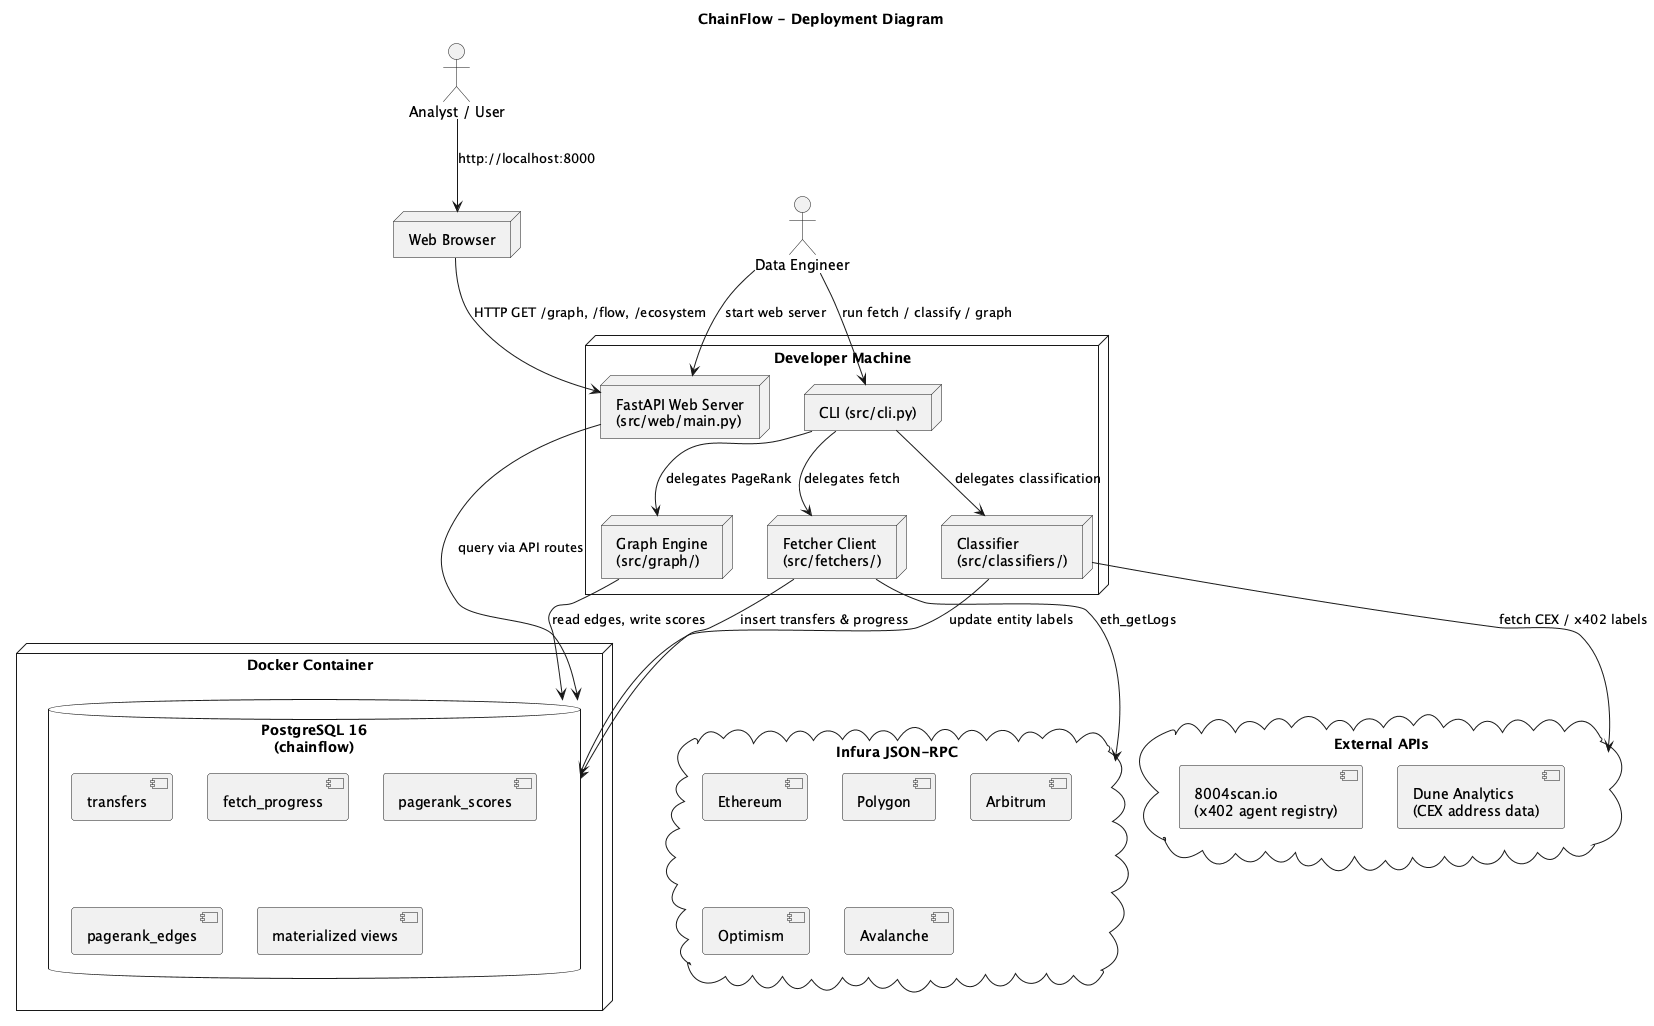
\includegraphics[width=0.85\textwidth]{figures/deployment_diagram.png}
    \caption{Deployment Diagram: ChainFlow System}
    \label{fig:deployment}
\end{figure}

% ============================================================
\chapter{IMPLEMENTATION AND TESTING}

\section{Implementation}

The implemented pipeline uses Python with PostgreSQL 16 and a Dockerized database runtime.
The web dashboard is served by Uvicorn/FastAPI.

\textbf{Key implementation decisions:}
\begin{itemize}
\item Switched from explorer APIs to Infura RPC for scalable, rate-limit-resilient event access.
\item Implemented adaptive chunk resizing (halving on overflow) to handle high-density block ranges
without manual intervention.
\item Inserted transfer data in batches with \texttt{ON CONFLICT DO NOTHING} for idempotent
re-runs.
\item Partitioned the \texttt{transfers} table by \texttt{network} for better query organization
and growth handling.
\item Applied classification as an \texttt{UPDATE}-only pass over existing rows, keeping
classification logic independent of ingestion.
\item Used \texttt{TEXT[]} arrays for entity class columns to support multi-label assignment
(e.g., an address may be both CEX and a bridge gateway).
\item Cached x402 agent addresses in YAML files to decouple periodic registry refreshes from
per-run classification.
\item Used NetworkX for graph construction and PageRank. Only the top-10,000 scored nodes per
network/token are persisted to keep storage and query overhead practical.
\item Materialized views are refreshed via a dedicated API endpoint
(\texttt{POST /api/ecosystem/refresh}) after each pipeline run.
\item The D3.js force graph in the PageRank Explorer fetches only the top-$N$ pre-ranked nodes
and their connecting edges from the database, making the visualization independent of full graph
traversal at render time.
\end{itemize}

\section{Testing}

Automated unit tests are not yet included in the repository. Validation was performed through
manual and integration-style checks:
\begin{itemize}
\item CLI argument validation for all four command groups.
\item Correct retrieval of latest block and latest processed DB block in auto mode.
\item Successful decoding of ERC-20 \texttt{Transfer} event fields from raw log payloads.
\item Duplicate-protection behavior through unique constraints and conflict handling.
\item Correct insertion of chunk metadata into \texttt{fetch\_progress}.
\item End-to-end verification that CEX/Bridge/x402 flags are correctly applied to transfers.
\item Sampling checks on PageRank output (verifying top addresses correspond to known exchange
hot wallets).
\item API response validation for all dashboard endpoints under different network/token filters.
\end{itemize}

\section{Deployment}

Deployment for development is lightweight, reproducible, and modular.

\subsection*{Environment Configuration}
Create a \texttt{.env} file in the project root:

\begin{verbatim}
# PostgreSQL
POSTGRES_DB=chainflow
POSTGRES_USER=chainflowuser
POSTGRES_PASSWORD=chainflowpass
POSTGRES_PORT=5432

# Infura credentials
INFURA_API_KEY=your_infura_key
INFURA_API_SECRET=your_infura_secret

# 8004scan.io credentials (for x402 agents)
SCAN_API_KEY=your_scan_key

# Dune Analytics (for CEX addresses)
DUNE_API_KEY=your_dune_key
\end{verbatim}

\subsection*{Database Setup}
\begin{enumerate}
    \item Start PostgreSQL container using Docker Compose:
    \begin{flushleft}
        \texttt{\small docker compose up -d}
    \end{flushleft}
    \item Execute SQL migration scripts in order:
\begin{verbatim}
psql -h localhost -U chainflowuser -d chainflow -f sql/01_create_tables.sql
psql -h localhost -U chainflowuser -d chainflow -f sql/02_create_indexes.sql
psql -h localhost -U chainflowuser -d chainflow -f sql/03_add_x402.sql
psql -h localhost -U chainflowuser -d chainflow -f sql/04_drop_class_labels.sql
psql -h localhost -U chainflowuser -d chainflow -f sql/05_event_entity_labels.sql
psql -h localhost -U chainflowuser -d chainflow -f sql/06_drop_old_class_labels.sql
psql -h localhost -U chainflowuser -d chainflow -f sql/07_double_class_labels.sql
psql -h localhost -U chainflowuser -d chainflow -f sql/08_pagerank.sql
psql -h localhost -U chainflowuser -d chainflow -f sql/09_pagerank_edges.sql
psql -h localhost -U chainflowuser -d chainflow -f sql/10_top_wallets_view.sql
psql -h localhost -U chainflowuser -d chainflow -f sql/11_ecosystem_views.sql
\end{verbatim}
\end{enumerate}

\subsection*{Running the Full Pipeline}
\begin{enumerate}
    \item Fetch transfer events:
    \begin{flushleft}
        \texttt{\small python3 src/cli.py fetch --network ethereum --auto}
    \end{flushleft}
    \item Classify addresses:
    \begin{flushleft}
        \texttt{\small python3 src/cli.py classify\_addresses --network ethereum}
    \end{flushleft}
    \item Classify x402 agents:
    \begin{flushleft}
        \texttt{\small python3 src/cli.py classify\_agents --network ethereum}
    \end{flushleft}
    \item Run PageRank:
    \begin{flushleft}
        \texttt{\small python3 src/cli.py graph --network ethereum}
    \end{flushleft}
    \item Start the web dashboard:
    \begin{flushleft}
        \texttt{\small uvicorn src.web.main:app --host 0.0.0.0 --port 8000}
    \end{flushleft}
\end{enumerate}

% ============================================================
\chapter{RESULTS}

\section{Data Collection}

The ChainFlow database currently holds \textbf{3,466,862 transfer events} collected across five
EVM-compatible networks. Table~\ref{tab:network_token} shows the real distribution by network
and token.

\begin{table}[H]
\centering
\caption{Transfer event counts by network and token (actual database counts)}
\label{tab:network_token}
\begin{tabular}{|l|r|r|r|r|r|}
\hline
\textbf{Network} & \textbf{USDT} & \textbf{USDC} & \textbf{DAI} & \textbf{XAUT} & \textbf{Total} \\\hline
Ethereum   & 643,605 & 503,879 & 13,256 & 3,560 & 1,164,300 \\\hline
Arbitrum   & 134,243 & 475,941 &  6,057 &     0 &   616,241 \\\hline
Polygon    & 191,104 &  85,371 & 328,392 &    0 &   604,867 \\\hline
Avalanche  & 144,699 & 386,929 &  30,642 &    0 &   562,270 \\\hline
Optimism   & 110,357 & 368,355 &  40,472 &    0 &   519,184 \\\hline
\textbf{Total} & \textbf{1,224,008} & \textbf{1,820,475} & \textbf{418,819} & \textbf{3,560} & \textbf{3,466,862} \\\hline
\end{tabular}
\end{table}

Notable observations:
\begin{itemize}
\item USDC dominates across the dataset (52.5\% of all events), driven by high activity on
Arbitrum, Avalanche, and Optimism.
\item DAI shows an unusual concentration on Polygon (328,392 out of 418,819 DAI events, or 78\%),
reflecting Polygon's historically strong DAI ecosystem.
\item Ethereum holds the largest single-network share (33.6\%) with the most diverse token
distribution including XAUT (gold-backed).
\item The block range coverage spans: Ethereum blocks 24.6M--25.3M, Polygon/Avalanche blocks
10M--88M, Arbitrum blocks 100M--471M, Optimism blocks 100M--152M.
\end{itemize}

\section{Address Classification Results}

Table~\ref{tab:classification} summarizes the classification coverage across networks.

\begin{table}[H]
\centering
\caption{Address classification results by network}
\label{tab:classification}
\begin{tabular}{|l|r|r|r|r|r|}
\hline
\textbf{Network} & \textbf{Total Tx} & \textbf{CEX Tx} & \textbf{Bridge Tx} & \textbf{x402 Tx} & \textbf{Regular} \\\hline
Ethereum  & 1,164,300 & 46,386 (4.0\%) & 44,939 (3.9\%) & 5,964 (0.5\%) & $\sim$91.6\% \\\hline
Arbitrum  &   616,241 & 10,853 (1.8\%) & 28,127 (4.6\%) & 3,180 (0.5\%) & $\sim$93.1\% \\\hline
Polygon   &   604,867 & 12,433 (2.1\%) & 11,830 (2.0\%) & 5,761 (1.0\%) & $\sim$95.0\% \\\hline
Avalanche &   562,270 &  7,166 (1.3\%) & 13,744 (2.4\%) & 5,743 (1.0\%) & $\sim$95.3\% \\\hline
Optimism  &   519,184 &  5,261 (1.0\%) & 19,512 (3.8\%) & 3,691 (0.7\%) & $\sim$94.5\% \\\hline
\end{tabular}
\end{table}

Key findings from classification:
\begin{itemize}
\item Ethereum has the highest absolute CEX and Bridge activity, consistent with its role as the
primary settlement layer.
\item Bridge transfers are proportionally higher on L2s (Arbitrum 4.6\%, Optimism 3.8\%), where
cross-chain bridging is a primary on-ramp/off-ramp mechanism.
\item x402 AI agent activity is present across all five networks (7--12 unique agent addresses
per network), with Polygon and Avalanche showing the highest relative share (1.0\%).
\end{itemize}

\section{Web Dashboard}

The ChainFlow web dashboard is operational and accessible at \texttt{http://localhost:8080}
after starting the FastAPI server. All three analysis tools -- PageRank Explorer, Flow Explorer,
and Ecosystem Overview -- are functional and connected to the live database. Materialized views
ensure that the Ecosystem Overview renders with sub-second response times regardless of
database size.

% ============================================================
\chapter{CONCLUSION}

This project delivered ChainFlow, a complete end-to-end system for stablecoin flow analysis on
EVM-compatible blockchains. The system progressed through all three planned phases:

\begin{enumerate}
\item \textbf{Fetch Phase:} A reliable, resumable ERC-20 event extraction pipeline collecting
3,466,862 transfer events across five networks and four tokens.
\item \textbf{Analysis Phase:} Address classification (CEX, Bridge, Mint/Burn) and x402 AI
agent identification, followed by directed transfer graph construction and weighted PageRank
computation.
\item \textbf{Reporting Phase:} The ChainFlow interactive dashboard, providing three views --
PageRank Explorer, Flow Explorer, and Ecosystem Overview -- backed by pre-computed database
results and materialized views.
\end{enumerate}

The project makes several concrete contributions:
\begin{itemize}
\item A scalable, transparent, and fully reproducible blockchain data collection pipeline.
\item A labeled stablecoin transfer dataset covering five major EVM networks.
\item A first-of-its-kind segmentation of x402 AI agent activity within the stablecoin
transfer ecosystem.
\item An interactive analysis dashboard that integrates graph theory, entity classification,
and network-level statistics in a single self-contained system.
\end{itemize}

\textbf{Remaining limitations:}
\begin{itemize}
\item Automated unit tests are absent. Integration-style manual checks were used throughout.
\item Classification coverage is incomplete by design; regular wallet addresses are classified
by exclusion. CEX and Bridge label sources (Dune Analytics queries) may not be fully up-to-date.
\item The block range collected for Ethereum (24.6M--25.3M, approximately 640k blocks) is
relatively short compared to the chain's history; longer windows would yield richer graph structure.
\item The 10,000-node cap on stored PageRank results excludes a large fraction of addresses.
\end{itemize}

\textbf{Future work directions:}
\begin{itemize}
\item Add automated test coverage (unit tests for decode logic, integration tests for DB inserts).
\item Expand Ethereum block range coverage; continue fetching across all networks.
\item Improve address labeling by integrating additional classification sources (DeFiLlama,
Arkham, on-chain contract introspection).
\item Add temporal flow analysis: sliding-window PageRank and flow pattern tracking over time.
\item Extend the dashboard with cross-chain flow comparison views and address cluster visualization.
\end{itemize}

\bibliographystyle{plain}
\bibliography{references}

\appendix
\chapter{COMMAND REFERENCE}

\section*{Data Ingestion}
\begin{itemize}
\item Automatic fetch (from last DB block to chain tip):
\begin{flushleft}
    \texttt{python3 src/cli.py fetch --network ethereum --auto}
\end{flushleft}
\item Manual fetch (specific block range):
\begin{flushleft}
    \texttt{python3 src/cli.py fetch --network polygon --manual --start 50000000 --end 50100000}
\end{flushleft}
\end{itemize}

\section*{Address Classification}
\begin{itemize}
\item Classify CEX/Bridge/Mint-Burn addresses:
\begin{flushleft}
    \texttt{python3 src/cli.py classify\_addresses --network ethereum}
\end{flushleft}
\item Update x402 agent file from registry and classify:
\begin{flushleft}
    \texttt{python3 src/cli.py classify\_agents --network ethereum --update}
\end{flushleft}
\end{itemize}

\section*{Graph Analysis}
\begin{itemize}
\item Run PageRank for all tokens on a network:
\begin{flushleft}
    \texttt{python3 src/cli.py graph --network ethereum --save}
\end{flushleft}
\item Run PageRank for a specific token:
\begin{flushleft}
    \texttt{python3 src/cli.py graph --network ethereum --token USDT --top 20}
\end{flushleft}
\end{itemize}

\section*{Web Dashboard}
\begin{itemize}
\item Start the FastAPI server:
\begin{flushleft}
    \texttt{uvicorn src.web.main:app --host 0.0.0.0 --port 8000}
\end{flushleft}
\item Refresh materialized views after a pipeline run:
\begin{flushleft}
    \texttt{curl -X POST http://localhost:8000/api/ecosystem/refresh}
\end{flushleft}
\end{itemize}

\section*{Infrastructure}
\begin{itemize}
\item Start PostgreSQL container:
\begin{flushleft}
    \texttt{docker compose up -d}
\end{flushleft}
\item Run schema migration scripts:
\begin{flushleft}
    \texttt{psql -h localhost -U chainflowuser -d chainflow -f sql/01\_create\_tables.sql}
\end{flushleft}
\end{itemize}

\end{document}
